\documentclass[oneside,openany,headings=optiontotoc,11pt,numbers=noenddot]{scrreprt}

\usepackage[a4paper]{geometry}
\usepackage[utf8]{inputenc}
\usepackage[T1]{fontenc}
\usepackage{lmodern}
\usepackage[ngerman]{babel}
\usepackage{ngerman}

\usepackage[onehalfspacing]{setspace}

\usepackage{fancyhdr}
\usepackage{fancybox}

\usepackage{rotating}
\usepackage{varwidth}

%Struktogramme
\usepackage[german,curves]{struktex}

\usepackage{pdflscape}
\usepackage{changepage}
\usepackage{graphicx}
\usepackage[bottom]{footmisc}
\usepackage{transparent}
\usepackage{graphbox}
\graphicspath{
	{Pics/PDFs/}
	{Pics/JPGs/}
	{Pics/PNGs/}
}
\usepackage{caption}
\usepackage{wrapfig}
\usepackage{marginnote}
\usepackage{tabularx}
\usepackage{dashrule}
\usepackage{soulutf8}
\usepackage{hhline}
%arydshln suppresses vertical lines in table
%\usepackage{arydshln}
\usepackage{multirow}
\usepackage{enumerate}
\usepackage[hidelinks]{hyperref}
\usepackage{listings}

\usepackage[table]{xcolor}
\usepackage{array}
\usepackage{enumitem,amssymb,amsmath}
\usepackage{interval}
\usepackage{cancel}
\usepackage{stmaryrd}
\usepackage{wasysym}
\usepackage{polynom}
\usepackage{diagbox}
\usepackage{dashrule}
\usepackage{framed}
\usepackage{mdframed}
\usepackage{karnaugh-map}
\usepackage{pdfpages}

\usepackage{blindtext}

\usepackage{eso-pic}

\usepackage{amssymb}
\usepackage{eurosym}

\usepackage[pages=some]{background}
\pagestyle{headings}
\renewcommand{\headrulewidth}{0.2pt}
\renewcommand{\footrulewidth}{0.2pt}
\newcommand*{\underdownarrow}[2]{\ensuremath{\underset{\overset{\Big\downarrow}{#2}}{#1}}}
\setlength{\fboxsep}{5pt}
\newcommand{\explainBelow}[3]{\underbrace{#1}_{\parbox{\widthof{#3}}{\footnotesize\raggedright #2}}}
\newcommand{\explainAbove}[3]{\overbrace{#1}^{\parbox{\widthof{#3}}{\footnotesize\raggedright #2}}}
\newcommand\footnoteref[1]{\protected@xdef\@thefnmark{\ref{#1}}\@footnotemark}


% Codestyle defined
\definecolor{codegreen}{rgb}{0,0.6,0}
\definecolor{codegray}{rgb}{0.5,0.5,0.5}
\definecolor{codepurple}{rgb}{0.58,0,0.82}
\definecolor{backcolour}{rgb}{0.95,0.95,0.92}
\definecolor{deepgreen}{rgb}{0,0.5,0}
\definecolor{darkblue}{rgb}{0,0,0.65}
\definecolor{mauve}{rgb}{0.40, 0.19,0.28}
\colorlet{exceptioncolour}{yellow!50!red}
\colorlet{commandcolour}{blue!60!black}
\colorlet{numpycolour}{blue!60!green}
\colorlet{specmethodcolour}{violet}

%Neue Spaltendefinition
\newcolumntype{L}[1]{>{\raggedright\let\newline\\\arraybackslash\hspace{0pt}}m{#1}}
\newcolumntype{M}{>{\centering\arraybackslash}X}
\newcommand{\cmnt}[1]{\ignorespaces}
%Textausrichtung ändern
\newcommand\tabrotate[1]{\rotatebox{90}{\raggedright#1\hspace{\tabcolsep}}}

%Intervall-Konfig
\intervalconfig {
	soft open fences
}

%Bash
\lstdefinestyle{BashInputStyle}{
	language=bash,
	basicstyle=\small\sffamily,
	backgroundcolor=\color{backcolour},
	columns=fullflexible,
	backgroundcolor=\color{backcolour},
	breaklines=true,
}
%Java
\lstdefinestyle{JavaInputStyle}{
	language=Java,
	backgroundcolor=\color{backcolour},
	aboveskip=1mm,
	belowskip=1mm,
	showstringspaces=false,
	columns=flexible,
	basicstyle={\footnotesize\ttfamily},
	numberstyle={\tiny},
	numbers=none,
	keywordstyle=\color{purple},,
	commentstyle=\color{deepgreen},
	stringstyle=\color{blue},
	emph={out},
	emphstyle=\color{darkblue},
	emph={[2]rand},
	emphstyle=[2]\color{specmethodcolour},
	breaklines=true,
	breakatwhitespace=true,
	tabsize=2,
}
%Python
\lstdefinestyle{PythonInputStyle}{
	language=Python,
	alsoletter={1234567890},
	aboveskip=1ex,
	basicstyle=\footnotesize,
	breaklines=true,
	breakatwhitespace= true,
	backgroundcolor=\color{backcolour},
	commentstyle=\color{red},
	otherkeywords={\ , \}, \{, \&,\|},
	emph={and,break,class,continue,def,yield,del,elif,else,%
		except,exec,finally,for,from,global,if,import,in,%
		lambda,not,or,pass,print,raise,return,try,while,assert},
	emphstyle=\color{exceptioncolour},
	emph={[2]True,False,None,min},
	emphstyle=[2]\color{specmethodcolour},
	emph={[3]object,type,isinstance,copy,deepcopy,zip,enumerate,reversed,list,len,dict,tuple,xrange,append,execfile,real,imag,reduce,str,repr},
	emphstyle=[3]\color{commandcolour},
	emph={[4]ode, fsolve, sqrt, exp, sin, cos, arccos, pi,  array, norm, solve, dot, arange, , isscalar, max, sum, flatten, shape, reshape, find, any, all, abs, plot, linspace, legend, quad, polyval,polyfit, hstack, concatenate,vstack,column_stack,empty,zeros,ones,rand,vander,grid,pcolor,eig,eigs,eigvals,svd,qr,tan,det,logspace,roll,mean,cumsum,cumprod,diff,vectorize,lstsq,cla,eye,xlabel,ylabel,squeeze},
	emphstyle=[4]\color{numpycolour},
	emph={[5]__init__,__add__,__mul__,__div__,__sub__,__call__,__getitem__,__setitem__,__eq__,__ne__,__nonzero__,__rmul__,__radd__,__repr__,__str__,__get__,__truediv__,__pow__,__name__,__future__,__all__},
	emphstyle=[5]\color{specmethodcolour},
	emph={[6]assert,range,yield},
	emphstyle=[6]\color{specmethodcolour}\bfseries,
	emph={[7]Exception,NameError,IndexError,SyntaxError,TypeError,ValueError,OverflowError,ZeroDivisionError,KeyboardInterrupt},
	emphstyle=[7]\color{specmethodcolour}\bfseries,
	emph={[8]taster,send,sendMail,capture,check,noMsg,go,move,switch,humTem,ventilate,buzz},
	emphstyle=[8]\color{blue},
	keywordstyle=\color{blue}\bfseries,
	rulecolor=\color{black!40},
	showstringspaces=false,
	stringstyle=\color{deepgreen}
}

\lstset{literate=%
	{Ö}{{\"O}}1
	{Ä}{{\"A}}1
	{Ü}{{\"U}}1
	{ß}{{\ss}}1
	{ü}{{\"u}}1
	{ä}{{\"a}}1
	{ö}{{\"o}}1
}

% Neue Klassenarbeits-Umgebung
\newenvironment{worksheet}[3]
% Begin-Bereich
{
	\newpage
	\sffamily
	\setcounter{page}{1}
	\ClearShipoutPicture
	\AddToShipoutPicture{
		\put(55,761){{
				\mbox{\parbox{385\unitlength}{\tiny \color{codegray}BBS I Mainz, #1 \newline #2
						\newline #3
					}
				}
			}
		}
		\put(455,761){{
				\mbox{\hspace{0.3cm}
\includegraphics[width=0.2\textwidth]{../../logo.pdf}}
			}
		}
	}
}
% End-Bereich
{
	\clearpage
	\ClearShipoutPicture
}

\geometry{left=1.50cm,right=1.50cm,top=2.50cm,bottom=0.50cm,includeheadfoot}
\pagestyle{empty}

\begin{document}
		\begin{worksheet}{Lernbereich 5}{Lernabschnitt: Mikrocontroller}{Berechnungen - Strom, Spannung und Widerstand}
			\begin{framed}
				\noindent
				\tiny{Die Aufgaben sind entnommen aus:
					\begin{itemize}
						\item Grafe, H./Loose, J./Kühn, H.: \textit{Grundlagen der Elektrotechnik - Band 1}: Gleichspannungstechnik - 4. durchgesehene Auflage - S. 126ff.
						\item Lindner, H. \textit{Physikalische Aufgaben} - 18. Auflage - S 144ff.
					\end{itemize}}\normalsize
				\textbf{Aufgabe 1:}\\
				In der Schaltung sind die Teilspannungen \(U_1\) bis \(U_3\) und sämtliche Ströme zu berechnen. Gegeben sind:\\
				\begin{minipage}[c]{0.48\textwidth}
					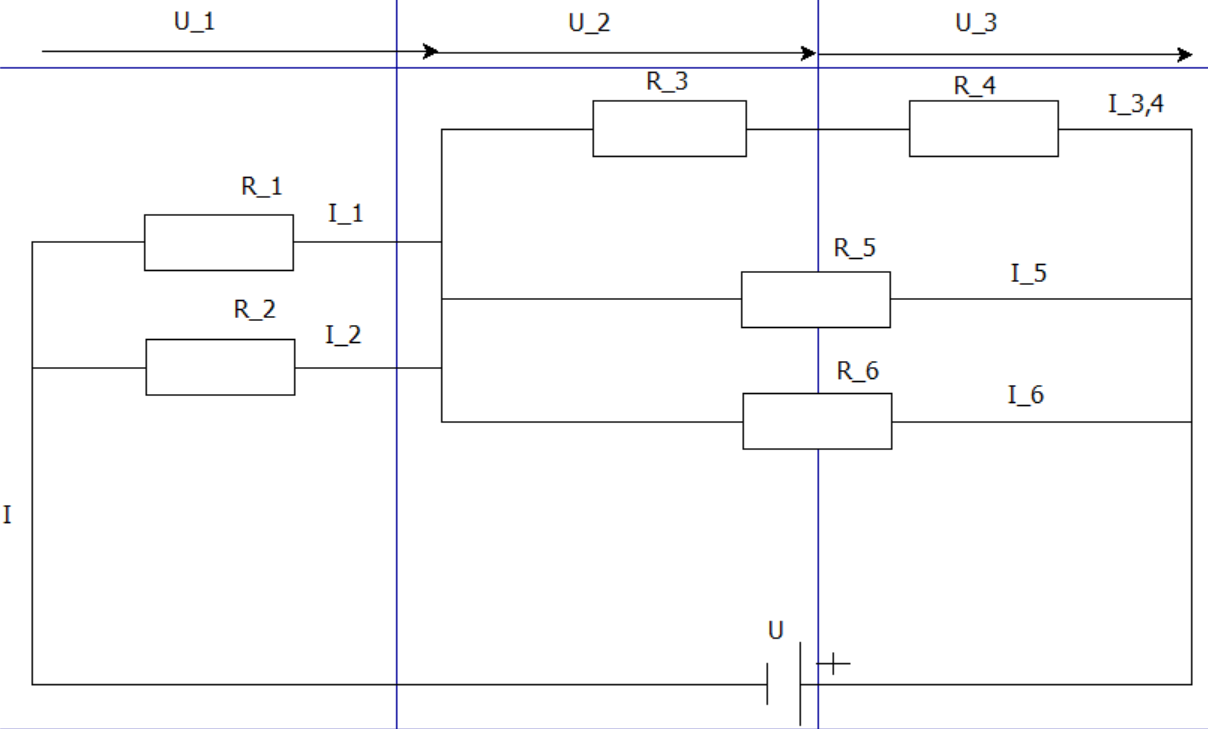
\includegraphics[width=0.98\textwidth]{../99_Bilder/A1.png}
				\end{minipage}
				\hfill
				\begin{minipage}[c]{0.24\textwidth}
					\begin{align*}
						U & = 220V\\
						R_1 & = 24\ \Omega\\
						R_2 & = 12\ \Omega\\
						R_3 & = 5\ \Omega
					\end{align*}
				\end{minipage}
				\hfill
				\begin{minipage}[c]{0.24\textwidth}
					\begin{align*}
						R_4 & = 8\ \Omega\\
						R_5 & = 17\ \Omega\\
						R_6 & = 26 \Omega
					\end{align*}
				\end{minipage}\\
				\par\noindent
				\textbf{Aufgabe 2:}\\
				Von der Schaltung sind gegeben:\\
				\begin{minipage}{0.48\textwidth}
					\begin{align*}
						U & = 4\ V\\
						R_r & = 100\ \Omega\\
						R_1 & = 200\ \Omega\\
						I_2 & = 8\ mA\\
						I_3 & = 2\ mA
					\end{align*}
				\end{minipage}
				\hfill
				\begin{minipage}{0.5\textwidth}
					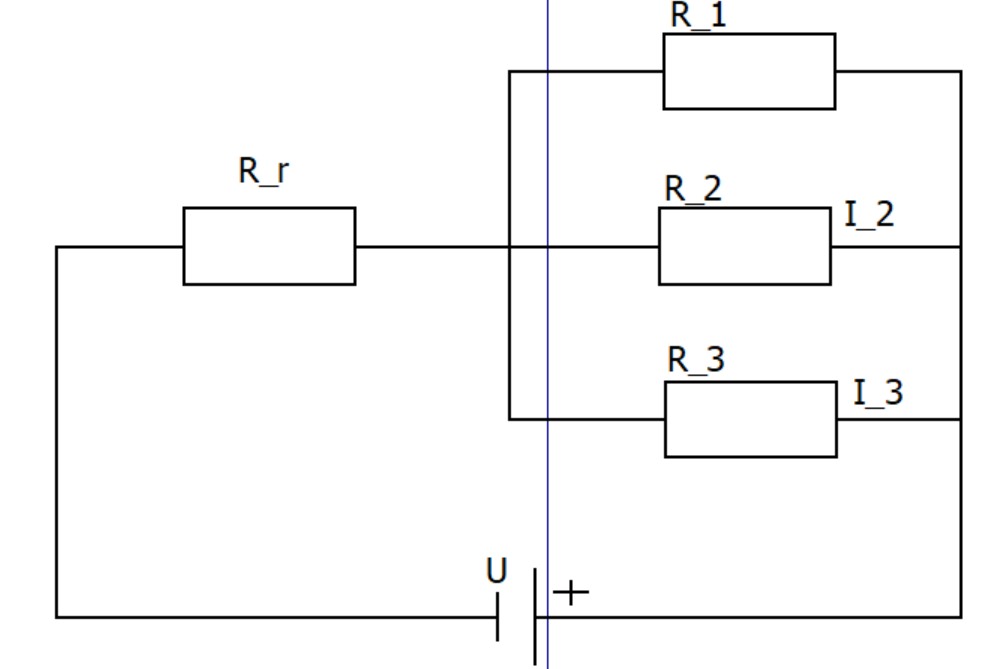
\includegraphics[width=0.98\textwidth]{../99_Bilder/A2.png}
				\end{minipage}\\
				\par\noindent
				\textbf{Aufgabe 3:}\\
				\begin{minipage}{0.58\textwidth}
					Wie groß muss \(R_2\) gewählt werden, wenn \(R_1 = 750\ \Omega\) ist und der Gesamtwiderstand \(R_g = 350\ \Omega\) betragen soll?
				\end{minipage}
				\hfill
				\begin{minipage}{0.38\textwidth}
					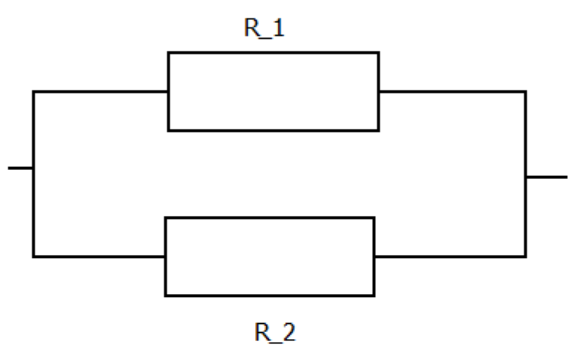
\includegraphics[width=0.98\textwidth]{../99_Bilder/A3.png}
				\end{minipage}\\
				\par\noindent
				\textbf{Aufgabe 4:}\\
				\begin{minipage}{0.58\textwidth}
					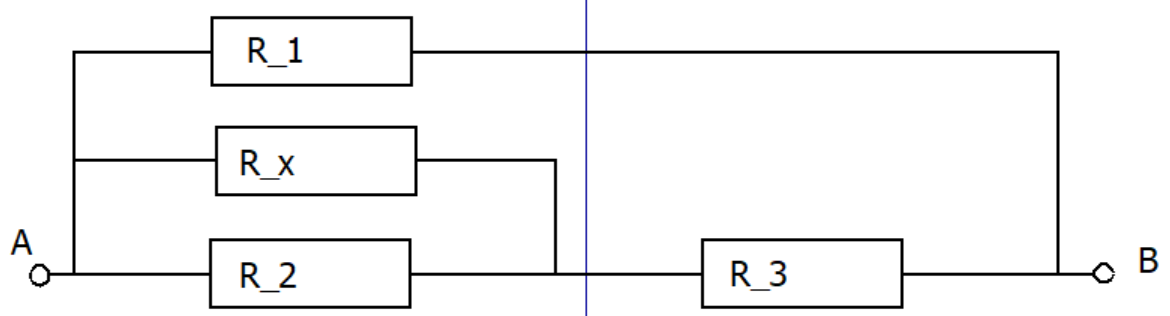
\includegraphics[width=0.98\textwidth]{../99_Bilder/A4.png}
				\end{minipage}
				\hfill
				\begin{minipage}{0.38\textwidth}
					Wie groß muss der Widerstand \(R_x\) gewählt werden, damit der Gesamtwiderstand zwischen den Klemmen A und B den Betrag \(R_{AB} = 7\ \Omega\) hat.
				\end{minipage}\\
				\par\noindent
				\textbf{Aufgabe 5:}\\
				Schaltet man zu einem widerstand \(R_1\) einen zweiten \(R_2\) parallel, so beträgt der Gesamtwiderstand nur noch \(\frac{R_1}{5}\).\\
				Wie groß ist das Verhältnis \(\frac{R_1}{R_2}\)?\\
				\par\noindent
				\tiny{Die nachfolgenden Aufgaben sind aus den Übungen von Alexander Veith übernommen.}\normalsize\\
				\textbf{Aufgabe 6:}\\
				\begin{enumerate}[label=(\alph*)]
					\item Der Ausgang eines \(\mu\)Cs darf maximal mit einem Strom von \(40mA\) belastet werden.\\
					Welchen Widerstandswert darf eine Last haben (maximal oder minimal)?
					\item Der Ausgang eines \(\mu\)Cs darf maximal mit einen Strom von \(30mA\) belastet werden.\\
					Welchen Widerstandswert darf eine Last haben (maximal oder minimal), wenn an dem Ausgang eine Spannung von \(4V\) anliegt?
					\item Am Ausgang eines \(\mu\)Cs (5V, max. Belastung \(40mA\)) sollen drei Lasten mit jeweils einer Leistung von \(70mW\) parallel angeschlossen werden.\\
					Ist dies zulässig?
					\item Der Ausgang eines \(\mu\)Cs darf maximal mit einem Strom von \(30mA\) belastet werden.\\
					Welchen Widerstandswert darf eine Last haben (maximal oder minimal), wenn an dem Ausgang eine Spannung von \(6V\) anliegt?
					\item Am Ausgang eines \(\mu\)Cs (\(6V\), max. Belastung \(30mA\)) sollen drei Lasten mit jeweils einer Leistung von \(10mW\) parallel angeschlossen werden.\\
					Ist das zulässig? Wie viele dieser Lasten sind maximal erlaubt?
				\end{enumerate}
				\par\noindent
				\textbf{Aufgabe 7:}\\
				Eine LED it \(U_{LED} = 2,2V\) und \(I_{LED} =  20mA\) soll an eine Spannung von insgesamt \(5V\) betrieben werden.
				\begin{enumerate}[label=(\alph*)]
					\item Berechnen Sie den notwendigen Vorwiderstand und wählen Sie passend aus der Tabelle \(E12\) aus.
					\item Wie groß ist die Verlustleistung am Vorwiderstand?
				\end{enumerate}
				\par\noindent
				\textbf{Aufgabe 8:}\\
				Eine LED mit \(U_{LED} = 2,4V\) und \(I_{LED} = 0,022A\) soll an eine Spannung von insgesamt \(10V\) angeschlossen werden.
				\begin{enumerate}[label=(\alph*)]
					\item Berechnen Sie den notwendigen Vorwiderstand und wählen Sie passend aus der Tabelle \(E24\) aus.
					\item Wie groß ist ungefähr die Verlustleistung am Vorwiderstand?
				\end{enumerate}
				\par\noindent
				\textbf{Aufgabe 9:}\\
				Eine LED mit \(U_{LED} = 2,4V\) und \(I_{LED} = 20mA\) soll an eine Spannung von 5V betrieben werden.
				\begin{enumerate}[label=(\alph*)]
					\item Berechnen Sie den notwendigen Vorwiderstand und wählen Sie passend aus der Tabelle \(E12\) aus.
					\item Wie groß ist die Verlustleistung am Vorwiderstand?
				\end{enumerate}
				\par\noindent
				\textbf{Aufgabe 10:}\\
				Zwei in Reihe geschaltete LEDs mit jeweils \(U_{LED} = 2,4V\) und \(I_{LED} = 20mA\) sollen an einer Spannung von \(10V\) betrieben werden.
				\begin{enumerate}[label=(\alph*)]
					\item Berechnen Sie den notwendigen Vorwiderstand und wählen Sie passend aus der Tabelle \(E24\) aus.
					\item Wie groß ist die Verlustleistung am Vorwiderstand?
				\end{enumerate}
				\par\noindent
				\textbf{Aufgabe 11:}\\
				Zwei in Reihe geschaltete LEDs mit jeweils \(U_{LED} = 2,2V\) und \(I_{LED} = 24mA\) sollen an einer Spannung von \(10V\) betrieben werden.
				\begin{enumerate}[label=(\alph*)]
					\item Berechnen Sie den notwendigen Vorwiderstand und wählen Sie passend aus der Tabelle \(E12\) aus.
					\item Wie groß ist die Verlustleistung am Vorwiderstand?
				\end{enumerate}
				\par\noindent
				\rule{0.98\textwidth}{0.1pt}\\
				\par\noindent
				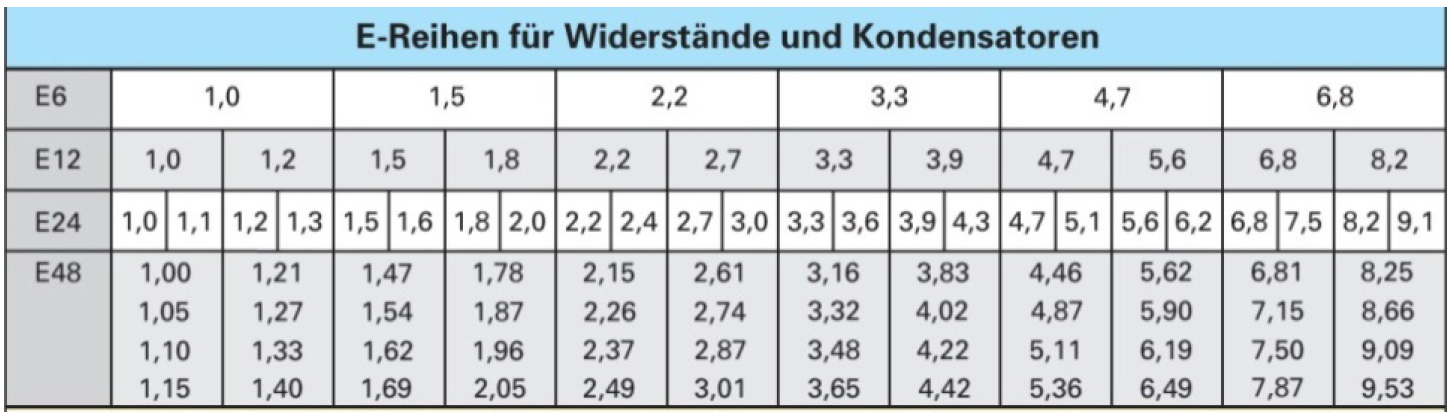
\includegraphics[width=0.98\textwidth]{../99_Bilder/eReihe.png}
			\end{framed}
		\end{worksheet}	
\end{document}